\section{Methodik}
Für die Realisation und das erreichen des Ziels musste ein Konkretes vorgehen und ein Grundsätzliche Architektur definiert werden. Hierfür spielten verschiedene Faktoren eine Rolle, welche im nachfolgenden beleuchtet werden.

\subsection{Allgemeiner Aufbau}
Da die Applikation von Grund auf entwickelt wird, wird der Allgemeine Aufbau von den beiden Entwicklern Maximilian Seitz und Michael Mican definiert. Der betreuende Professor Prof. Dr. Peter Faber fungiert während der Entwicklung als Project Owner.

\subsubsection{Projekt Vorgaben}
Das Kernziel bestand in der Visualisierung von Vektoren im Dreidimensionalen Raum, welche den gemessenen Magnetnischenfluss eine flüssigen Metalls in Echtzeit auf eine Sichverschlossene Kokille zu projizieren. Dies soll möglichst unkompliziert und Zugänglich ermöglicht werden, um auch kurzfristig ohne großen aufwand Besuchern und Gästen eine Benutzung zu ermöglichen. Aus diesem Grund wird eine Webbasierte Lösung umgesetzt, da so in der Theorie nur eine Webseite mit dem Smartphone besucht werden muss um die Applikation zu benutzen. In vorangehenden ähnlichen Projekten wurde deutlich, dass Übersichtlichkeit hierbei eine große Rolle spielt. Zur Lösung des Problems soll eine frei Bewegliche ebene mit definierbarer dicke im Vektorfeld bewegt werden können um so nur nach einem Ausschnitt der Daten intuitiv Filtern zu können. Da die Daten direkt vor Ort gemessen und Sicherheitsrelevant besitzen soll es möglich sein die Daten in einem lokalen Netzwerk zu hosten um eine grundlegende IT - Sicherheit zu gewährleisten. Hierbei treten jedoch unter Berücksichtigung der anderen vorgaben Probleme auf.


%\begin{itemize}
%	\item Was will man visualiseren?
%	\begin{itemize}
%		\item Magnetischerfluss von Flüssigem metall in Kokille
%		\item Soll dabei helfen die einlaufgeschwindigkeit zu regulieren
%	\end{itemize}
%	
%	\item Geschlossenes netzwerk
%	\begin{itemize}
%		\item Kein Internet zugriff
%	\end{itemize}
%	
%	\item Möglichkeit der filterung der visuellen Ergebnisse
%	\item Soll auf Handy ohne Einstellungen laufen\\
%		("Einfach auf website gehen und LETS GOOOOOO")
%\end{itemize}


\subsubsection{Probleme und Abweichungen von den Vorgaben}
Seit einigen Jahren können sogenannte \grqq Powerful Features\grqq\space nurnoch von Seiten mit \grqq Secure origin\grqq , also zertifizierte HTTPS Seiten, genutzt werden. Diese Entscheidung fiel auf Grundlage technischer fortschritte, die es aus sicherheitsrelevanter Sicht nicht mehr vertretbar machte Funktionen wie Beispielsweise Geräteposition und Kamera von klassischen nicht zertifizierten HTTP Seiten zu ermöglichen (vgl. The Chromium Projects \cite{CameraHTTPSOnly}). Die Datenübermittlung, welche von HTTPS genutzt wird macht es Angreifern schwerer solche kritische Daten ab zugreifen. Somit ist es erforderlich eine HTTPS Webseite für die Applikation zu nutzen. Daher wird die Frontend Seite über Github distributiert, wodurch sie ein HTTPS Zertifikat einer anerkannten Zertifizierungsstelle erwirbt. Diesem vertrauen Webbrowser Standardmäßig wodurch eine Manuelle Einstellung am Endgerät nicht getätigt werden muss.\\
Dieses vorgehen führt zu einem weiterem Problem. Seit Anfang 2020 ermöglicht es Google Chrome standardmäßig nicht mehr HTTP quellen auf einer HTTPS Seite zu benutzen (vgl. Chromium Blog \cite{MixedSourcesPolicy}). Unter Berücksichtigung der Sicherheits vorgaben durch den Project Owner ist eine Einstellung am Endgerät unumgänglich. Hierfür gibt es zwei möglichkeiten.\\
Einerseits kann, um den lokalen Daten host HTTP Server benutzen zu können, die Einstellung \grqq Allow unsecure content\grqq\space in den Browser Einstellungen auf \grqq Allow\grqq\space gesetzt werden. Hierdurch wird die Mixed Content policy ignoriert und HTTP quellen können auch auf der Seite benutzt werden. In Chrome Desktop kann diese Option in den Webseiteneinstellungen gefunden werden. Auf einem Smarphone hingegen muss hierfür der interne Settings link \verb|"chrome://flags/#unsafely-treat-insecure-origin-as-secure"| genutzt werden (siehe Abbildung \ref{fig:insecureOriginsSettings}).\\
Die zweite Möglichkeit das Problem zu lösen erfordert eine eigene definierte HTTPS Zertifizierung des Daten Servers. Da diese Zertifizierung nicht via Internet geschehen kann muss hierfür ein eigenes Benutzerdefiniertes Zertifikat angelegt und am Endgerät, welches die Website aufruft, als bekanntes Zertifikat installiert werden.\\ 
Nach Abstimmung mit dem Project Owner wird das Problem bis auf weiteres bei der Entwicklung nicht berücksichtigt. Stattdessen wird sowohl das Frontend alsauch das backend mit Simulierten Daten im Internet mit validen HTTPS zertifikaten gehostet.

\begin{figure}
	\centering
	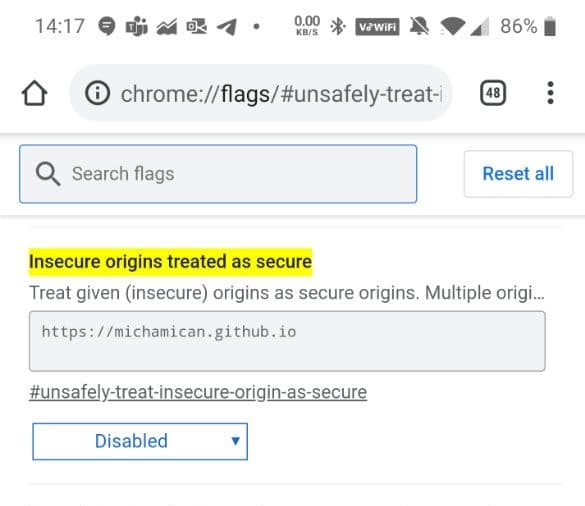
\includegraphics[width=.75\linewidth]{images/InsecureOriginsSettings}
	\caption{Allow insecure origin in Chrome mobile}
	\label{fig:insecureOriginsSettings}
\end{figure}

%\begin{itemize}
%	\item HTTPS erforderlich für kamera
%	\begin{itemize}
%		\item Lokaler Host Server braucht SSL zertifikat - Manuelle trustung des Zertifikats am handy unumgänglich
%	\end{itemize}
%	
%	\item HTTPS oder unsecured source Einstellung für backend kommunikation erforderlich
%	\item=> Für Beispielzwecke beides HTTPS via Internet
%\end{itemize}


\subsubsection{Komponenten}
\label{section:Komponenten}

Um Komponenten austauschbar zu machen, und Wiederverwendung davon zu
ermöglichen, wird eine Architektur mir einem Frontend und Backend
umgesetzt. Dabei übernimmt das Frontend die Visualisierung der Daten,
in der Form einer Website, die die Daten, welche Angezeigt werden,
von einem Server einholt, der das Backend bildet.

Dabei werden die Aufgaben so verteilt, dass das Frontend unabhängig
vom genauen Anwendungsgebiet ist, zu welchem ihm das Backend alle
Informationen über eine API zur Verfügung stellt.

Um dies zu Ermöglichen, wird die Funktionalität auf ihre abstrakten
Bestandteile reduziert, die dann vom Frontend unterstützt wird.
Diese Teile sind die Anzeige von einem Vektorfeld, und einem
3D-Modell der Umgebung, projiziert auf die echte Welt, durch die
Kamera. Synchronisierung findet hierzu über einen AR-Marker statt.
Diese Funktionalitäten sind die Voraussetzung, welche jedoch
erweitert werden, um das Nutzen der Anwendung zu erleichtern.
Jegliche solche Änderungen sind in Kapitel \ref{section:Frontend}
beschrieben. Die vorausgesetzten Kommunikationsschnittstellen werden
in Kapitel \ref{section:Backend} genauer beschrieben.

Durch diese Architektur, ist ein Austausch des Backends möglich,
was Visualisierung anderer Daten erlaubt. Diese Datenquellen können
beispielsweise Luftströme um ein Objekt anzeigen, zuvor aufgenommene
Daten wiedergeben, oder Abwärme simulieren. Das Frontend ist dazu
fähig auch solche Daten, mit den selben mitteln, an zu zeigen.

%\begin{itemize}
%	\item Backend vs. Frontend
%	\begin{itemize}
%		\item Frontend: AR visualisierung (allgemein)
%		\item Backend: Implementierungs spezifizierung
%		\item ziel: Frontend kann mit verschiedenen Backends genutzt werden
%	\end{itemize}
%\end{itemize}


\subsection{Visualisierung/Frontend}
\label{section:Frontend}
\FloatBarrier

Für das Anzeigen von Daten wird eine Website entwickelt, welche
für Smartphones optimiert wird. Diese Website bildet das, in Kapitel
\ref{section:Komponenten} eingeführte, Frontend der Anwendung.
Die hier umgesetzte Website fungiert als portable, und dynamisch
auslieferbare Applikation, die von einem Webservice, dem Backend,
Daten anfordert, um diese an zu zeigen.

\begin{figure}
	\centering
	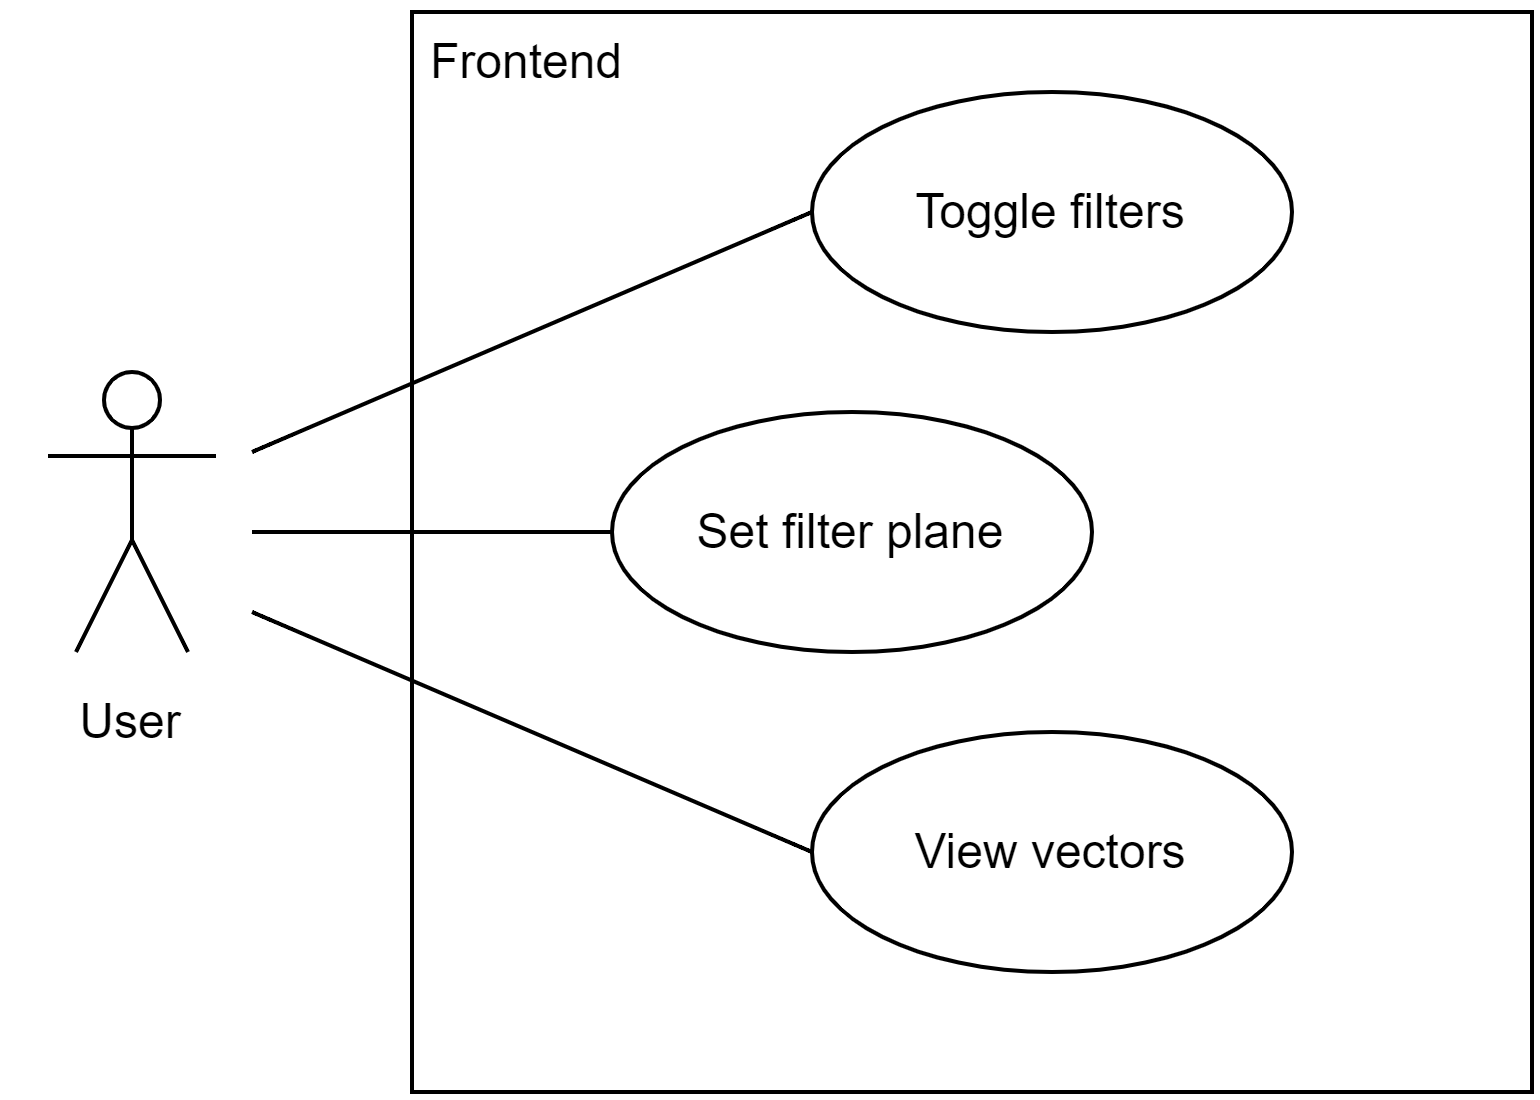
\includegraphics[width=.6\linewidth]{images/frontend/UseCases}
	\caption{Frontend use cases.}
	\label{fig:frontendUseCase}
\end{figure}

Abbildung \ref{fig:frontendUseCase} zeigt die Nutzungsmöglichkeiten
des Frontends. Es werden 3D-Vektoren als Pfeile dargestellt,
die abhängig von ihrer Länge eingefärbt sind. Dabei werden
Änderungen der Daten, in regelmäßigen abständen, angenommen. Diese
Änderungen werden abgefragt, jedoch liegt dabei der Fokus darin, die
Pfeile für den Nutzer erkennbar dar zu stellen, statt möglichst
Echtzeitdaten zu nutzen. Es wird zudem erlaubt die Vektoren auf eine
Örtlich begrenzte Gruppe ein zu schränken, wodurch nur diese
dargestellt wird. Um den Vektoren visuelle Referenzpunkte zu geben,
wird ein Grundgerüst geladen und angezeigt. Dieses Gerüst ist ein
unveränderliches 3D-Objekt, um das die Pfeile sich befinden.
Diese Szene wird über einen Kamerastream gezeichnet. Dabei wird
aus dem Bild ein, vom Backend definierter, Marker gesucht,
von welchem eine 3D-Position berechnet wird. Diese Position wird
genutzt, um die 3D-Szene zu positionieren, und sie in der echten
Welt zu ankern. Dies lässt die 3D-Szene als Erweiterung der echten
Welt erscheinen, und macht sie zur so genannten \grqq Augmented
Reality\grqq\space (vgl. AR.js Documentation \cite{ARjsDoc}).

Um virtuelle Objekte performant darzustellen, wird OpenGL genutzt.
Der Zugriff darauf wird von der JavaScript Bibliothek
\grqq Three.js\grqq\space übernommen. Als vereinheitlichte
Schnittstelle zur Echten Welt, wird \grqq AR.js\grqq , als
Erweiterung von \grqq Three.js\grqq\space genutzt.
\grqq AR.js\grqq\space steuert den Zugriff auf die Kamera des
Endgerätes, und erkennt darin den geladenen Marker. Für diesen
Marker wird ein virtuelles Gegenstück erzeugt, welches die
gleiche relative Größe und Position zur virtuellen Kamera hat,
wie dar physische Marker, zur physischen Kamera.

\begin{figure}
	\centering
	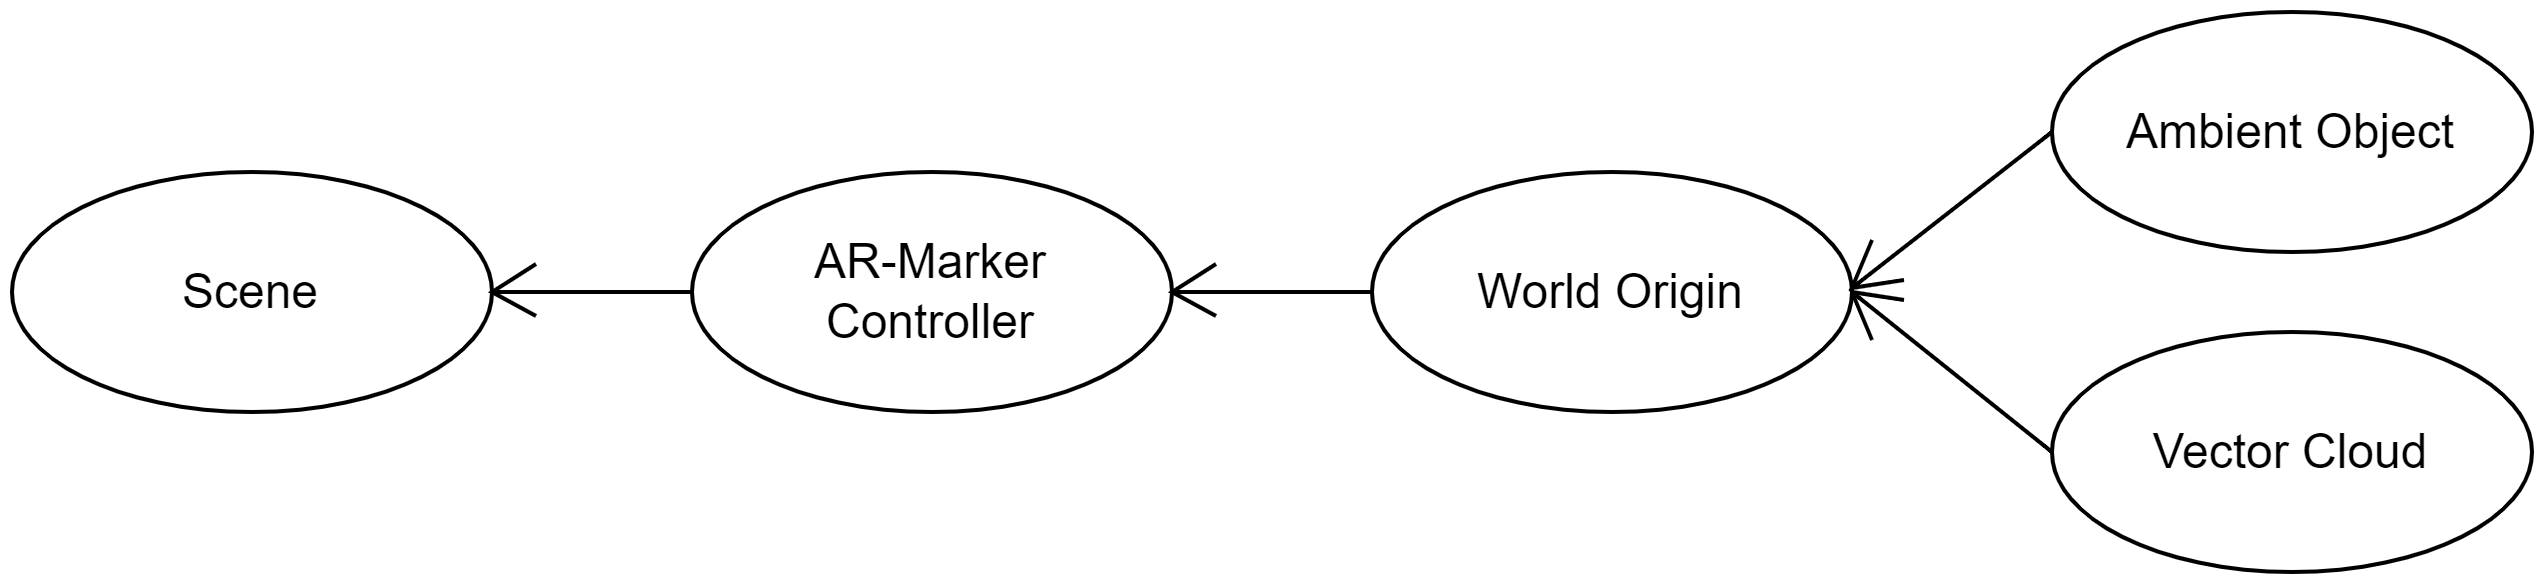
\includegraphics[width=1\linewidth]{images/frontend/SceneTree}
	\caption{Szenen-Baum des Frontends}
	\label{fig:SceneTree}
\end{figure}

Abbildung \ref{fig:SceneTree} zeigt den Szenen-Baum, der
Beschreibt wie die Objekte im der Szene voneinander beeinflusst
werden. Jedes Objekt erbt von seinem Vorfahren die Position und
Skalierung. Objekte sind hier nicht dringend mit einer graphischen
Darstellung verbunden. Solche Objekte werden \grqq Gruppen\grqq\space
genannt. Die \grqq Szene\grqq\space ist eine Gruppe, deren Nachkommen
angezeigt werden. Der \grqq AR-Marker Controller\grqq\space ist die
Gruppe, die von \grqq AR.js\grqq\space an die Kamera angepasst wird.
Alle Objekte, die teil der AR Darstellung sind, sind Nachkommen dieser
Gruppe. Da der Marker in Größe und Position, in Abhängigkeit des
logischen Koordinatenursprungs der echten Welt variiert, wird die
Gruppe \grqq World Origin\grqq\space angelegt. Bei einer Verschiebung
des Markers im Versuchsumfeld, kann der \grqq World Origin\grqq\space
gegenläufig, mit dem gleichen Betrag, verschoben werden, um dies zu
korrigieren. Diese Gruppe hat die angezeigten Objekte als Kinder.
Das ist einerseits das \grqq Ambient Object\grqq , welches zur
Orientierungshilfe dient, und andererseits eine \grqq Vector
Cloud\grqq , was eine Menge an Pfeil-Objekten ist, die angepasst
werden, um die Vektoren darzustellen, ohne regelmäßig neue Objekte
zu erstellen und zerstören.

%\begin{itemize}
%	\item Abbildung \ref{fig:frontendUseCase} zeigt
%		die Möglichkeiten des Frontends.
%	\begin{itemize}
%		\item Filtern
%		\item Anzeigen
%	\end{itemize}
%	
%	\item Three.js + AR.js
%	\begin{itemize}
%		\item OpenGL
%	\end{itemize}
%
%	\item Auswahl von Filter-Parametern
%	\item Object-Tree:
%	\begin{itemize}
%		\item Marker-Origin (wird von AR.js verschoben -> auf Marker in Quelle)
%		\begin{itemize}
%			\item Welt-Origin (korrigiert Marker verschiebung+rotation+skalierung von welt-origin)
%			\begin{itemize}				
%				\item Kokille Modell
%				\item Pfeile (10000 * ArrowHelper)
%				\item Filter-Box
%			\end{itemize}
%		\end{itemize}
%	\end{itemize}
%\end{itemize}



\subsection{Daten Bereitstellung/Backend}
\label{section:Backend}

Zur Bereitstellung der Daten wird eine REST API implementiert.
Über diese API kann das Frontend alle Usecase spezifischen Daten
abrufen (siehe Abbildung \ref{fig:backendUseCase}). Somit kann das
selbe Frontend durch eine einfach Änderung der API url an mehren
Orten verwendet werden. Alle Antworten der API sind in JSON codiert,
da JSON besser für dynamische Webapplikationen und einfachen
Datentransfer geeignet ist als andere ähnliche Datenformate wie
XML (vgl. Šimec \cite{comparisonJsonXml}). Die Vektordaten werden
als Array zurückgegeben. Jedes Vektorobjekt besitzt jeweils eine
x, y, z, xVec, yVec und zVec Property (Siehe Code \ref{code:VecJSON}).
Sie definieren den Fußpunkt des Vektors (x, y, z) und die Richtung
des Vektors (xVec, yVec, zVec).

\begin{codeblock}
	\begin{lstlisting}[
		language=json,
		caption={Aufbau der Vektordaten JSON},
		label={code:VecJSON}
	]
[
	{
		"x": float,
		"y": float,
		"z": float,
		"xVec": float,
		"yVec": float,
		"zVec": float
	}
]
	\end{lstlisting}
\end{codeblock}

Grundsätzlich müssen 2 wichtige Endpunkte implementiert werden und ein Endpunkt zur Datenbereitstellung verfügbar gemacht werden.
Der Datenbereitstellungs-Endpunkt hostet die eingangs erwähnten Usecase spezifischen statischen Dateien. Hierzu zählen die Model spezifischen Daten, welche die visuelle Representation und Texturierung der Kokille darstellen, die settings und Parameter für die Kamera und das Markerpattern und Informationen zu Positionierung und Skalierung der echten Kokille relativ zum marker.\\
Die beiden anderen Endpunkte bewegen sich um die tatsächlichen gemessenen Vektordaten. Sie bieten die Möglichkeit über eine GET Schnittstelle die Vektordaten zu holen und über eine weitere GET Schnittstelle die Metadaten dieser Vektoren, wie die Anzahl und die jeweiligen min und max x,y und z werte der Vektoren, zu beziehen. Darüber hinaus ist es möglich bei der Datenabfrage über Query Parameter einen Einheitsvektor und eine Distanz mitzugeben, welche eine Filterebene definiert, sodass nur Vektoren innerhalb der definierten Distanz von dieser Filterebene zurückgegeben werden.\\
Diese Endpunkte müssen anderen Seiten und Domänen abgefragt werden können. Aufgrund von Cross-Origin Resource Sharing Policies (CORS) ist hierfür ein spezielles Vorgehen erforderlich. Der Client sendet bei seiner Anfrage im \grqq Origin\grqq\space Header seine Domäne mit. Der Server muss diese Domäne akzeptieren und in seiner Antwort den \grqq Access-Control-Allow-Origin\grqq\space Header mit der jeweiligen Domäne oder einem \grqq *\grqq\space befüllen (vgl. Kesteren \cite{van2014cross}). Der hier implementierte backend Server gibt immer einen \grqq Access-Control-Allow-Origin\grqq\space Header mit dem Wert \grqq *\grqq\space zurück, wodurch jegliche Seiten und Domänen die Datenakquirieren können. Dies kann aber im Anwendungsfall aus sicherheitstechnischen Gründen geändert werden müssen.

\begin{figure}
	\centering
	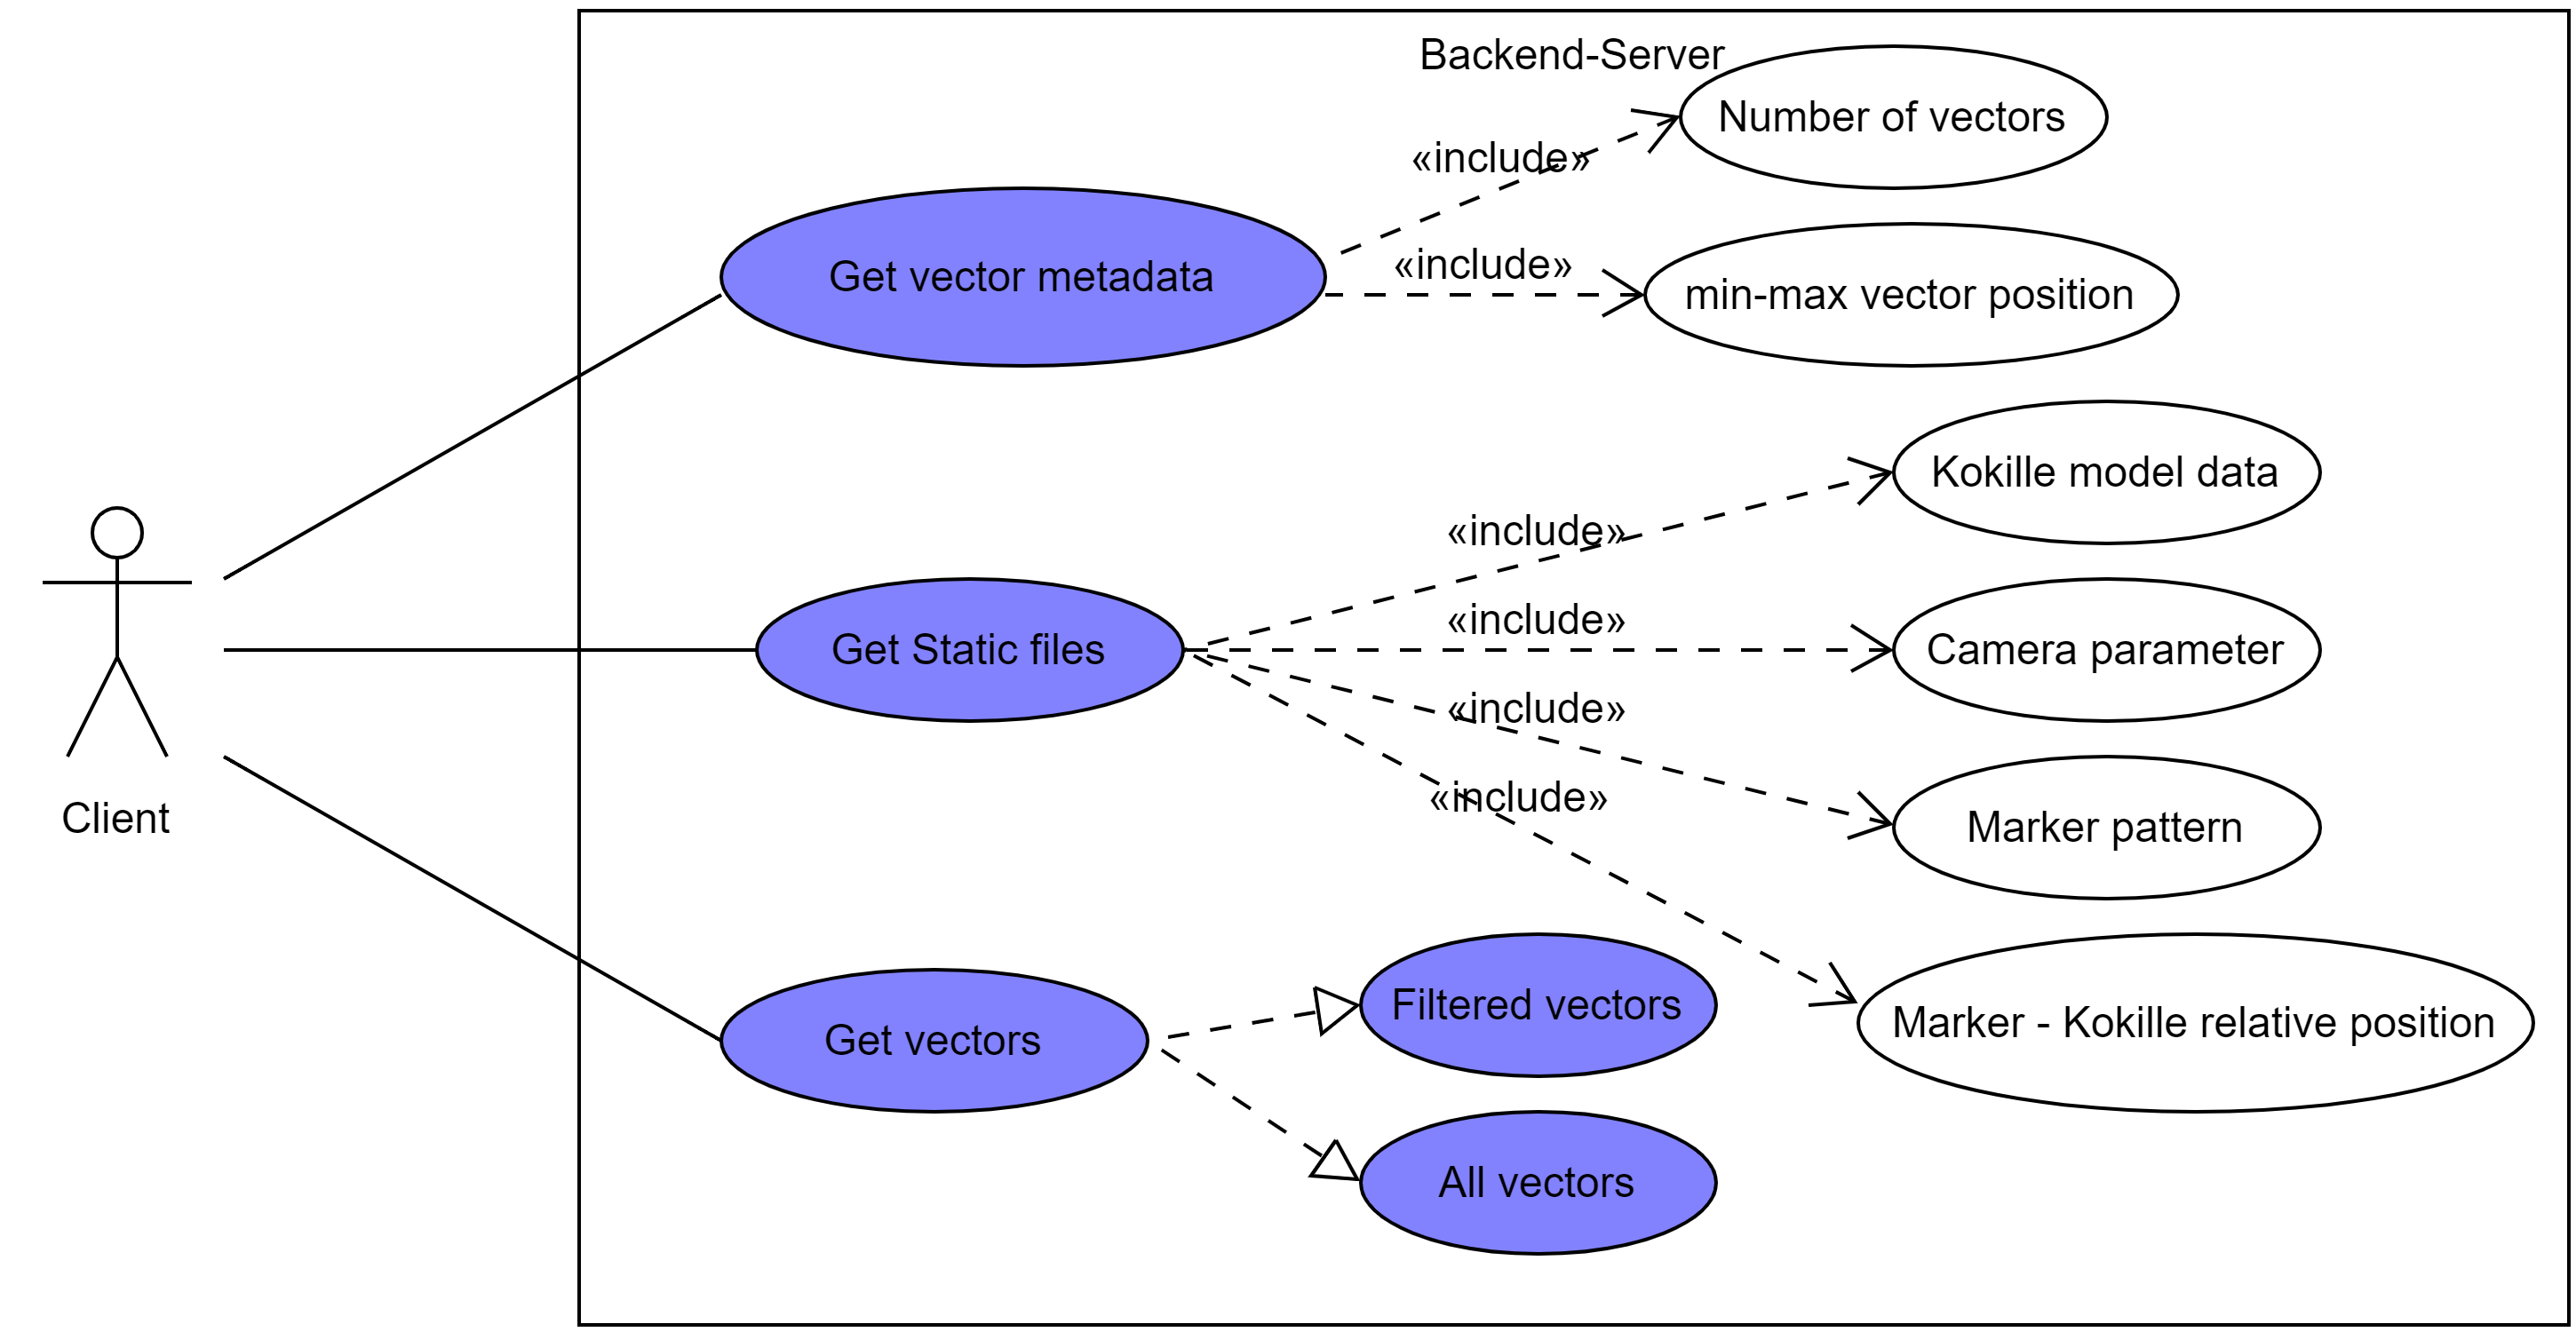
\includegraphics[width=1\linewidth]{images/backend/APIUseCases}
	\caption{API use cases.}
	\label{fig:backendUseCase}
\end{figure}


%\begin{enumerate}
%	\item REST (REST conforme endpunkte)
%	\item JSON (quote his paper)
%	\item Aufbau
%	\begin{itemize}
%		\item Architektur
%		\begin{itemize}
%			\item Endpunkte (evtl als diagram (Usecase))
%			\begin{itemize}
%				\item GET /api/data
%				\begin{itemize}
%					\item Gibt Vector Daten im JSON format zurück
%				\end{itemize}
%				
%				\item GET /api/data/v2
%				\begin{itemize}
%					\item Gibt Vector Daten im JSON format zurück und unterstützt filterung
%				\end{itemize}
%				
%				\item GET /api/data/meta
%				\begin{itemize}
%					\item Gibt Informationen über zur verfügung gestellte daten zurück
%					\item (anzahl vektoren im Datensatz, min \& max werte für axen)
%				\end{itemize}
%			\end{itemize}
%			
%			\item Hosten der Static files
%			\begin{itemize}
%				\item /hiro.patt
%				\item /kokilleTransformation.JSON
%				\item /positioning.JSON
%				\item /camera\_para.dat
%				\begin{itemize}
%					\item allgemeine camera parameter (von AR js mit ausgesendet)
%					\item idealterweise jede camera eigene parameter (utopie)
%				\end{itemize}
%				
%				\item /model
%				\begin{itemize}
%					\item /kokille.mtl
%					\item /kokille.obj
%				\end{itemize}
%			\end{itemize}
%		\end{itemize}
%			
%		\item CORS
%		\begin{itemize}
%			\item Nötig damit api von anderen websiten aufgerufen werden kann
%			\item Prinzip:
%			\begin{itemize}
%				\item Client schickt Origin Header mit
%				\item Wenn Origin zu der liste der zugelassenen Hosts ist wird bei der antwort der Allow-Origin Header gesetzt
%			\end{itemize}
%		\end{itemize}
%	\end{itemize}
%\end{enumerate}



